\documentclass[landscape]{slides}
\usepackage[landscape, margin=2cm]{geometry}
\usepackage{color}
\usepackage{bm}
\usepackage{graphicx}
\usepackage{hyperref}
\graphicspath{ {./img/} {./charts/} }



\title{Show and Tell: Skill Acquisition}
\author{Adam Johnson - me@adamj.eu}
\date{28th August 2013}

\begin{document}

\maketitle


\begin{slide}

    \textcolor{blue}{\Large{Skill Acquisition}}

    \begin{itemize}
        \item I have been re-learning a skill recently
        \item I tracked myself doing it
        \item This is the story...
    \end{itemize}

\end{slide}



\begin{slide}

    \textcolor{blue}{\Large{The Skill}}

    \begin{itemize}
        \item A puzzle for you...
    \end{itemize}

    % - something you did today
    % - you've been paid to do it
    % - you've probably never practiced it in your life

    % no, it's not making tea...

\end{slide}


\begin{slide}

    \textcolor{blue}{\Large{Typing!}}

    \centering

    
\includegraphics[height=10cm]{baby-nerd}

    (not me)

\end{slide}


\begin{slide}

    \textcolor{blue}{\Large{Motivation}}

    \begin{itemize}
        \item I'm a programmer - I have a lot of typing to do!
        \item Fear of RSI - both Mum and colleague have both been crippled by it
        % \item Always \emph{intended} to learn to touchtyping
        \item Stat: ``In the USA, carpal tunnel syndrome results in an average of \$30,000 in lifetime costs'' (Wikipedia)
    \end{itemize}

\end{slide}


\begin{slide}

    \textcolor{blue}{\Large{To business!}}

    \begin{itemize}
        \item Just need to grab some typing programs
        \item Get down to learning QWERTY the \emph{right} way!!
    \end{itemize}

\end{slide}


\begin{slide}

    \centering

    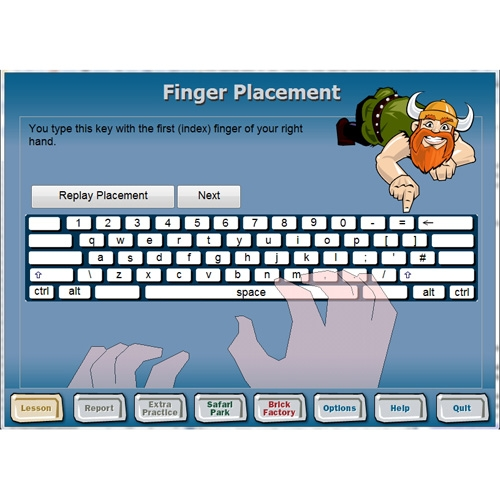
\includegraphics[height=19cm]{ten-thumbs}

\end{slide}


\begin{slide}

    \textcolor{blue}{\Large{Oh no....}}

\end{slide}

\begin{slide}
    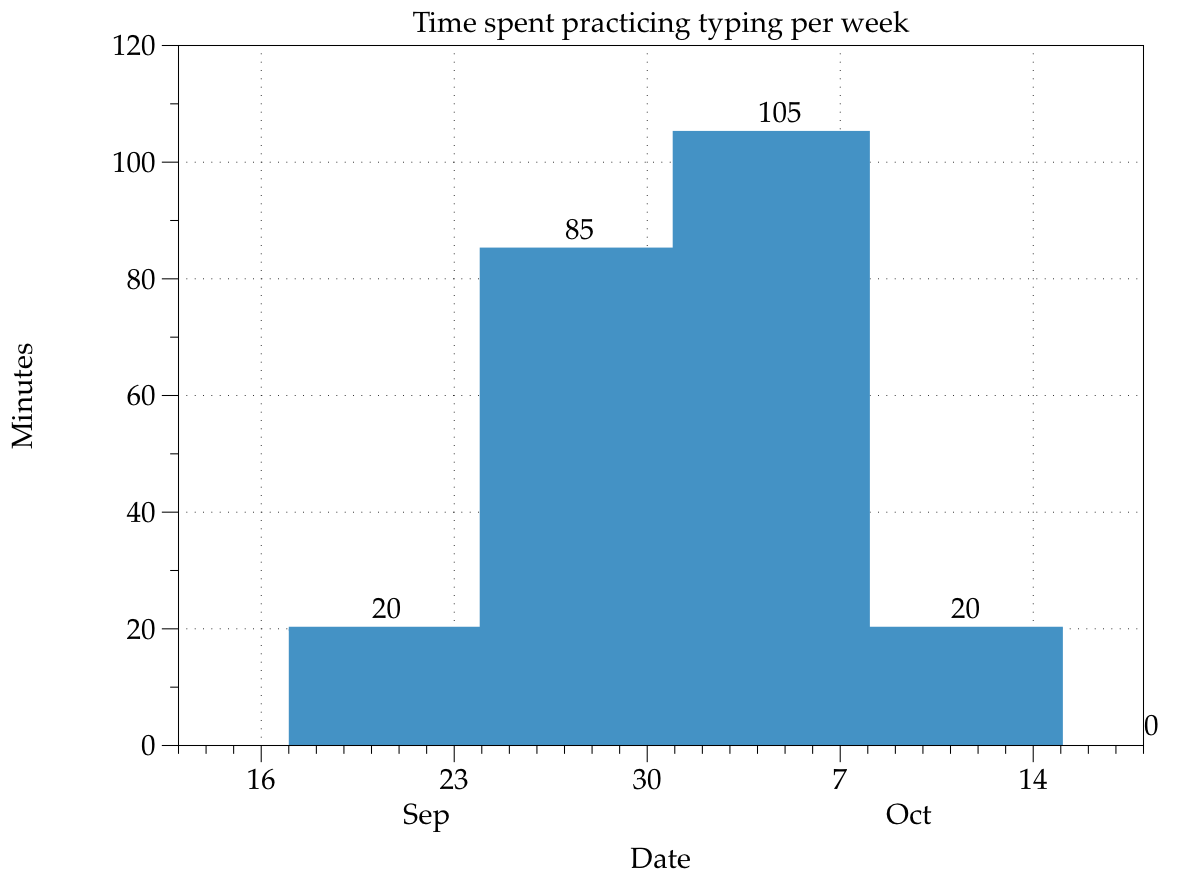
\includegraphics[width=\textwidth]{first-practice}
\end{slide}

\begin{slide}
    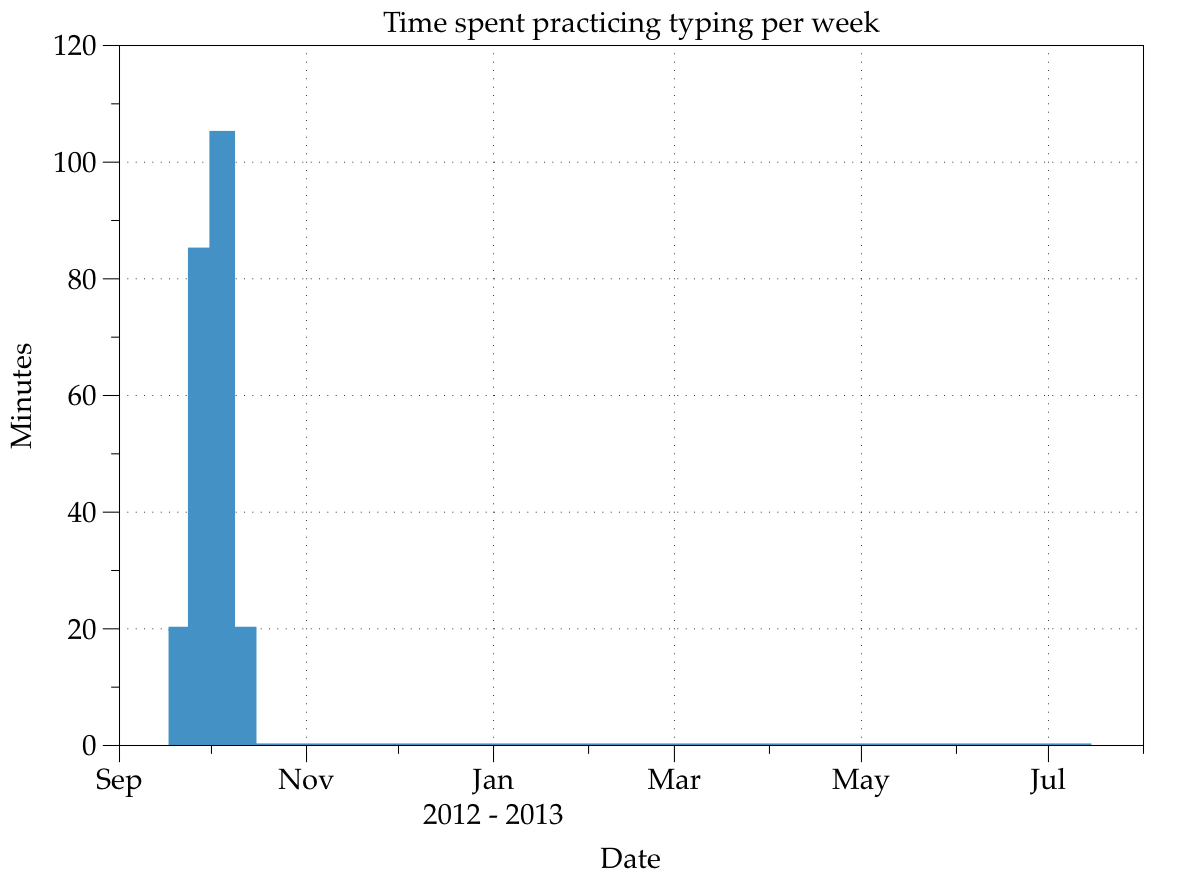
\includegraphics[width=\textwidth]{first-practice-long-tail}
\end{slide}


\begin{slide}

    \textcolor{blue}{\Large{Under-motivation}}

    \begin{itemize}
        \item Didn't know how long it would take
        \item Relative size of advantage
        \item Hard practicing QWERTY \emph{the right way} at night, then going back to old habits during the day
    \end{itemize}

\end{slide}


\begin{slide}

    \textcolor{blue}{\Large{So what changed?}}

    \begin{itemize}
        \item A book
    \end{itemize}

\end{slide}


\begin{slide}

    \textcolor{blue}{\Large{The First 20 Hours}}

    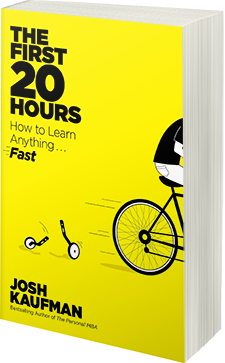
\includegraphics[height=10cm]{first20hours-cover}

    \begin{itemize}
        \item Josh Kaufman
    \end{itemize}

\end{slide}


\begin{slide}

    \textcolor{blue}{\Large{The First 20 Hours}}

    \begin{itemize}
        \item Learning a skill shouldn't take more than 20 hours to get to a good enough standard
        \item A couple chapters of general how-to, then one chapter on each skill he learnt with his method
        \item One of these was touchtyping... with `Colemak'
    \end{itemize}

\end{slide}


\begin{slide}

    \textcolor{blue}{\Large{QWERTY}}

    \centering
    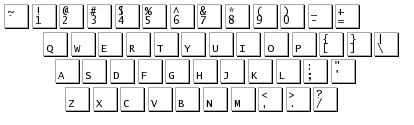
\includegraphics[width=20cm]{qwerty}

    \begin{itemize}
        \item Checkered past...
    \end{itemize}

\end{slide}


\begin{slide}

    \textcolor{blue}{\Large{Colemak}}

    \centering
    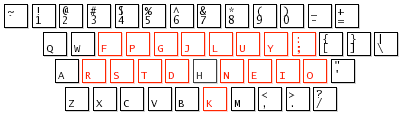
\includegraphics[width=20cm]{colemak-annot}

    \begin{itemize}
        \item Smooth future...
    \end{itemize}

\end{slide}


\begin{slide}

    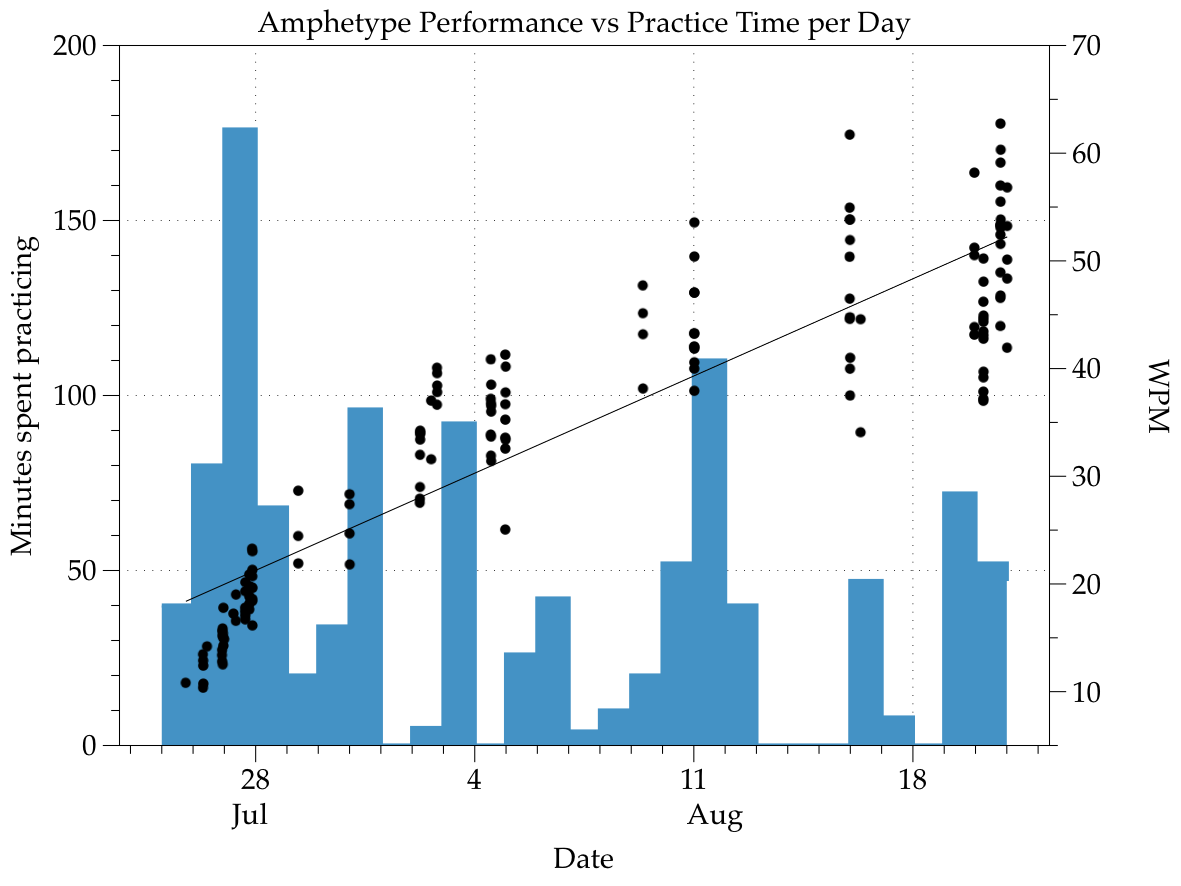
\includegraphics[width=\textwidth]{amphetype}

\end{slide}


\begin{slide}
    \textcolor{blue}{\Large{Thank you}}

    \begin{itemize}
        \item Slides on GitHub - \url{http://is.gd/adamIsDaBomb}
        \item Email me - \url{me@adamj.eu}
    \end{itemize}

\end{slide}


\end{document}
